% Auto-generated by generate_architecture.py
% Compile: pdflatex tee_qai_edge_architecture.tex
%
% CHANGELOG (Suzaki review alignment)
% ---------------------------------------------------------------------------
% [2025-06-21] Fix 1 — Move Decision Logic into REE zone (red fill).
%   Reason: Box was inside the TEE zone while labelled "REE-side", contradicting
%   the text and misleading reviewers about where policy/alert actions execute.
%
% [2025-06-21] Fix 2 — Merge Inference TA + Anomaly Scorer into one TEE box.
%   Reason: Two TEE boxes implied two runtime TAs / two secure-world stages;
%   implementation is a single Inference TA running one quantum-inspired C surrogate.
%
% [2025-06-21] Fix 3 — Remove Pi~5 hardware box from TEE; label Edge Gateway zone.
%   Reason: Platform hardware spans REE+TEE; placing Pi~5 inside TrustZone was wrong.
%
% [2025-06-21] Fix 4 — Rename "Management Agent" → "Gateway Orchestrator".
%   Reason: "Agent" triggered Agent-AI/IDS misinterpretation; component only coordinates REE I/O.
%
% [2025-06-21] Fix 5 — Add prototype status line under implementation assumptions.
%   Reason: Suzaki asked for Pi+OP-TEE evidence; figure must distinguish plan vs. demo.
% ---------------------------------------------------------------------------
\documentclass[tikz,border=10pt]{standalone}
\usepackage[T1]{fontenc}
\usepackage{lmodern}
\usepackage{xcolor}
\usepackage{tikz}
\usetikzlibrary{arrows.meta,calc,positioning,fit}

\definecolor{zonefill0}{HTML}{FFE0B2}
\definecolor{zonefill1}{HTML}{C8E6C9}
\definecolor{zonefill2}{HTML}{ECEFF1}
\definecolor{zonefill3}{HTML}{FFCDD2}
\definecolor{zonefill4}{HTML}{BBDEFB}
\definecolor{zonefill5}{HTML}{B3E5FC}
\definecolor{zonefill6}{HTML}{E0E0E0}

\tikzset{
  cmp/.style={draw=black!65, rounded corners=3pt, line width=0.7pt, fill=white,
    align=center, inner sep=5pt, minimum height=0.72cm, font=\small},
  zone/.style={draw=black!55, rounded corners=5pt, line width=0.85pt, inner sep=10pt, opacity=0.35},
  arr/.style={-{Latex}, line width=0.85pt, draw=black!70},
  trust/.style={-{Latex}, line width=0.9pt, draw=blue!60!black},
  deploy/.style={-{Latex}, line width=0.85pt, draw=orange!70!black, dashed},
  lbl/.style={font=\scriptsize, fill=white, inner sep=1pt, text=black!70},
  notebox/.style={draw=black!35, rounded corners=3pt, fill=white, font=\scriptsize,
    align=left, inner sep=5pt, text width=5cm},
  figtitle/.style={font=\bfseries\large, align=center, text width=0.88\linewidth},
  figsubtitle/.style={font=\small, align=center, text=black!65, text width=0.90\linewidth},
  bullets/.style={font=\small, align=left, text width=0.92\linewidth, anchor=north},
  flowdesc/.style={font=\small, align=left, text width=0.99\linewidth, anchor=north},
  rqdesc/.style={font=\footnotesize, align=left, text width=0.99\linewidth, anchor=north},
  impldesc/.style={font=\footnotesize, align=left, text width=0.99\linewidth, anchor=north},
}

\begin{document}
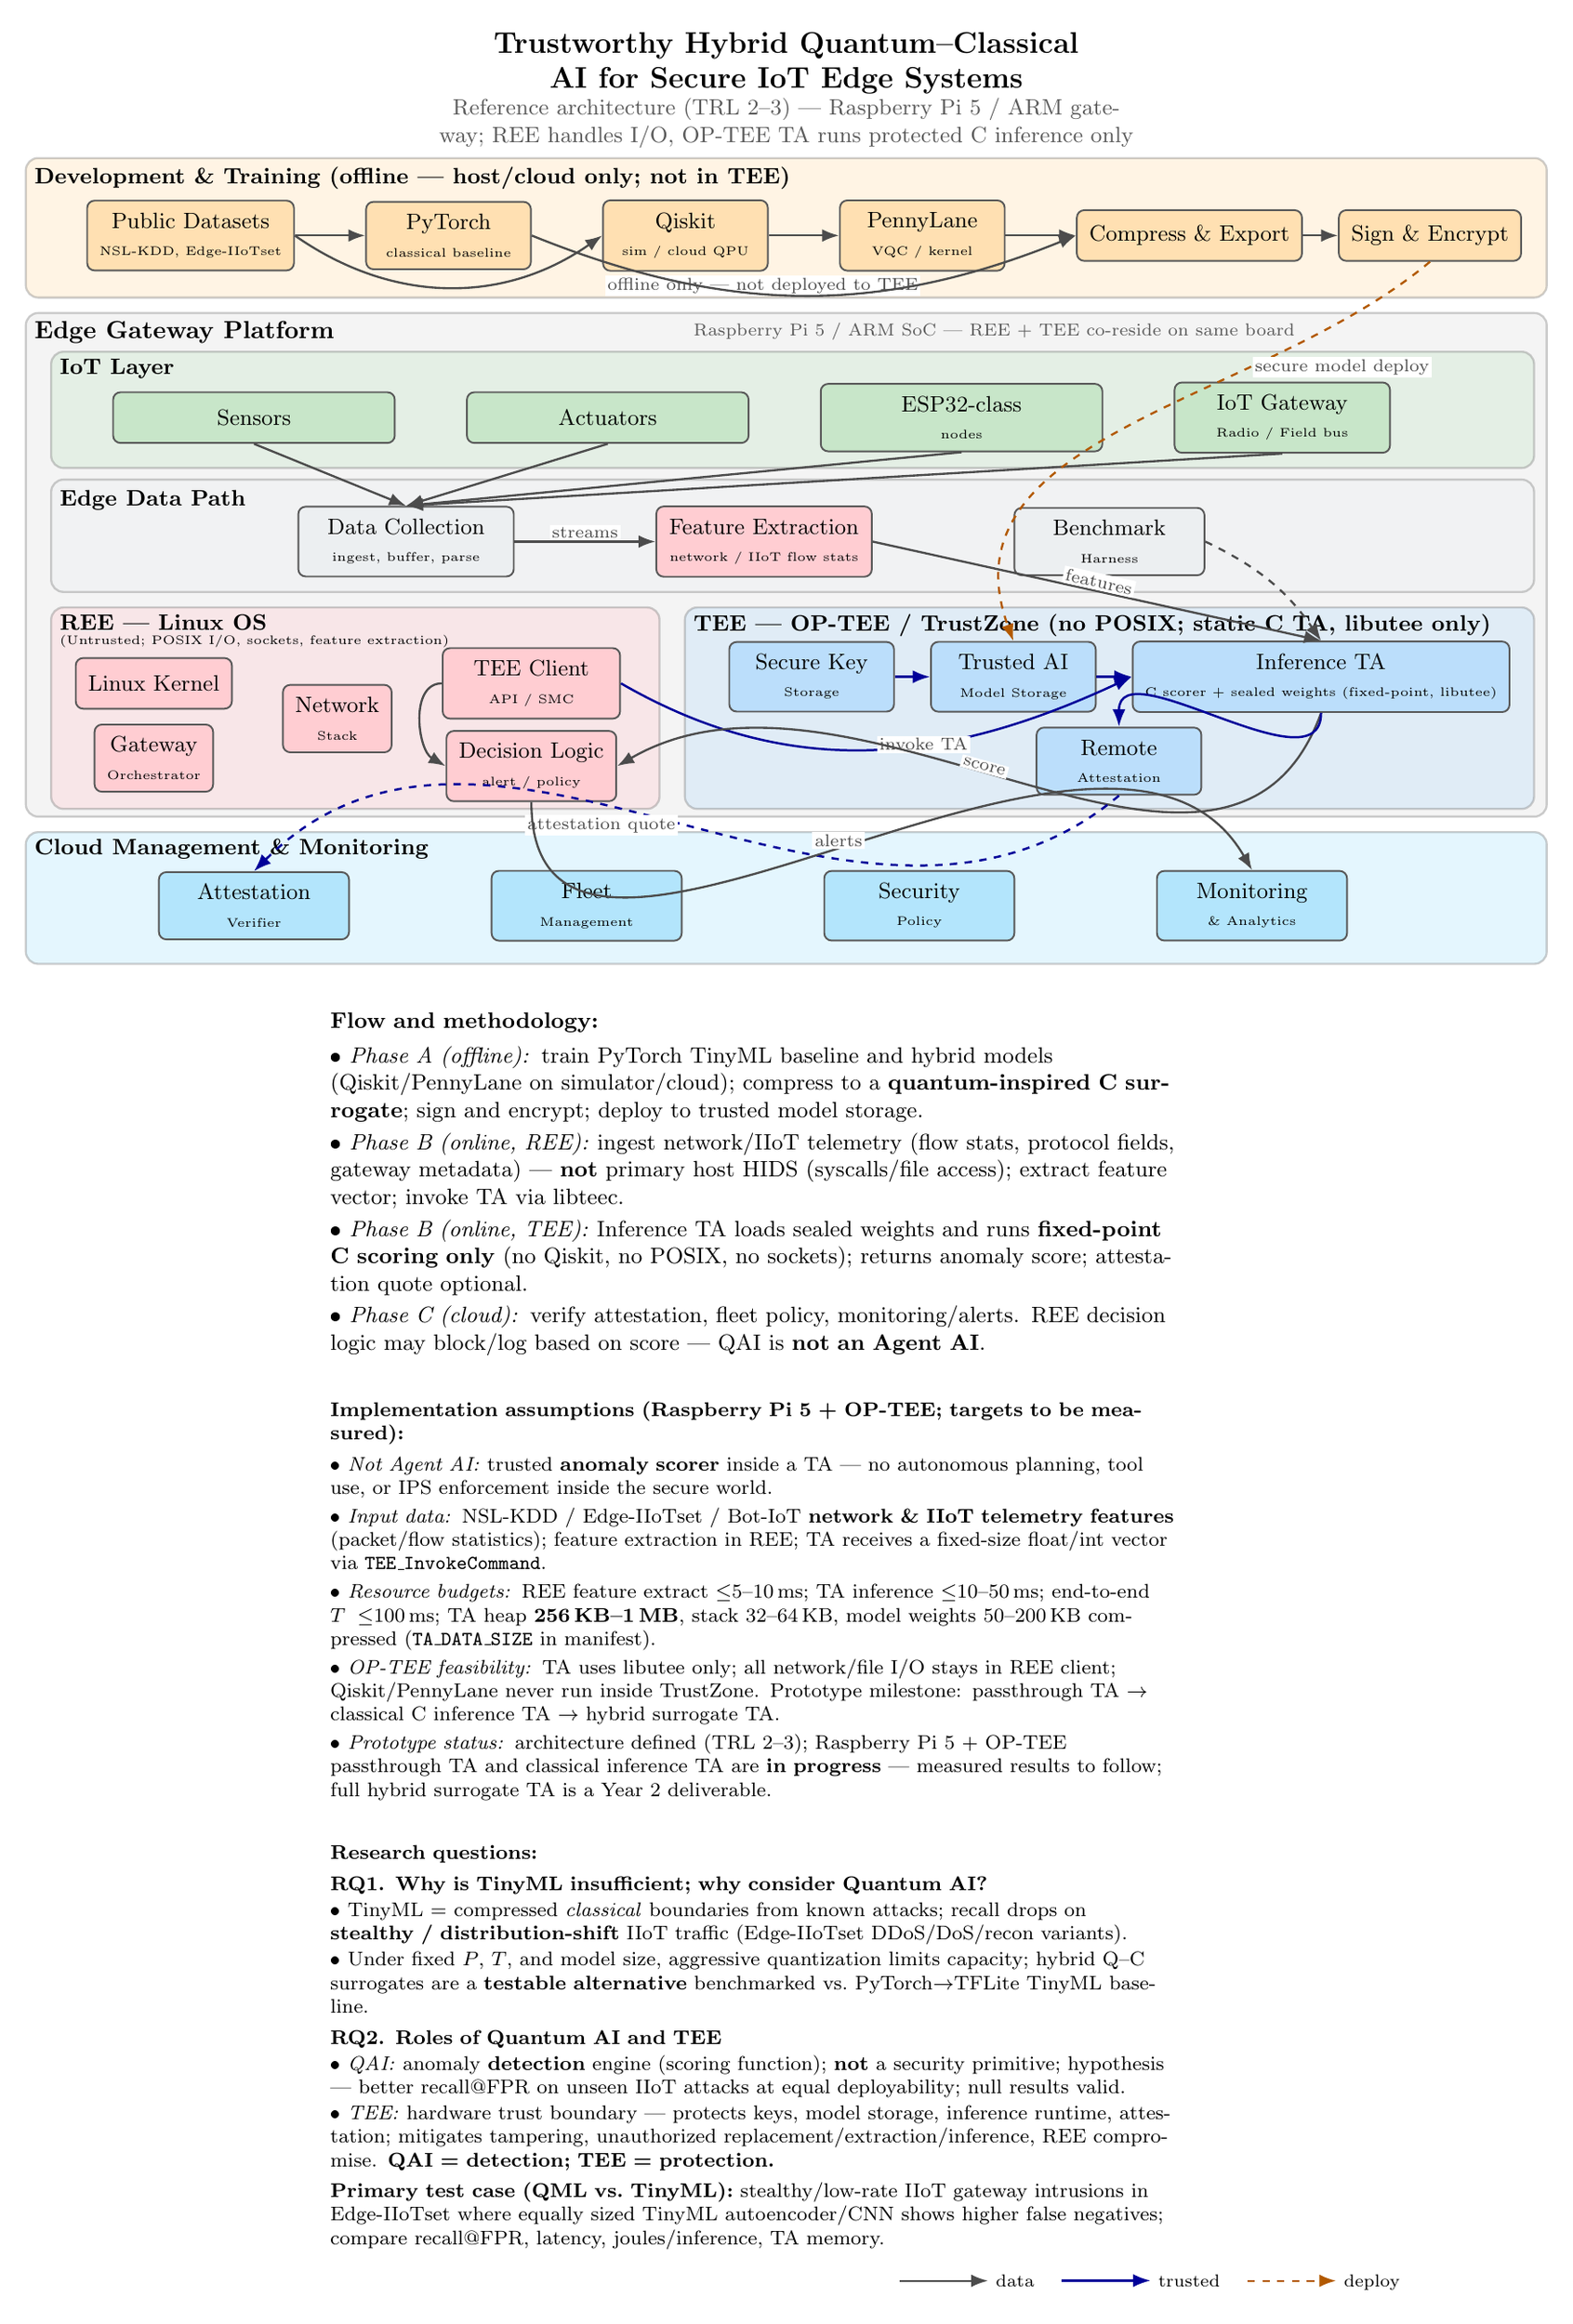
\begin{tikzpicture}[x=18.0cm, y=11.0cm]

\node[figtitle] at (0.50, 1.222) {Trustworthy Hybrid Quantum--Classical AI for Secure IoT Edge Systems};
\node[figsubtitle] at (0.50, 1.145) {Reference architecture (TRL~2--3) --- Raspberry Pi~5 / ARM gateway; REE handles I/O, OP-TEE TA runs protected C inference only};

\draw[zone, fill=zonefill0] (-0.10,0.920) rectangle (1.1,1.1);
\node[anchor=north west, font=\bfseries\small] at (-0.1,1.1) {Development \& Training (offline --- host/cloud only; not in TEE)};

\draw[zone, fill=zonefill6] (-0.1,0.25) rectangle (1.1,.9);
\node[anchor=north west, font=\bfseries] at (-0.1,0.9) {Edge Gateway Platform};
\node[anchor=north west, font=\scriptsize, text=black!65] at (0.42,0.898) {Raspberry Pi~5 / ARM SoC --- REE + TEE co-reside on same board};


\draw[zone, fill=zonefill1] (-0.08,0.70) rectangle (1.09,0.850);
\node[anchor=north west, font=\bfseries\small] at (-0.08,0.852) {IoT Layer};
\draw[zone, fill=zonefill2] (-0.08,0.540) rectangle (1.09,0.6850);
\node[anchor=north west, font=\bfseries\small] at (-0.08,0.682) {Edge Data Path};
\draw[zone, fill=zonefill3] (-0.08,0.260) rectangle (0.40,0.520);
\node[anchor=north west, font=\bfseries\small] at (-0.08,0.522) {REE --- Linux OS};
\node[anchor=north west, font=\tiny] at (-0.08,0.495) {(Untrusted; POSIX I/O, sockets, feature extraction)};
\draw[zone, fill=zonefill4] (0.420,0.260) rectangle (1.09,0.520);
\node[anchor=north west, font=\bfseries\small] at (0.42,0.522) {TEE --- OP-TEE / TrustZone (no POSIX; static C TA, libutee only)};
\draw[zone, fill=zonefill5] (-0.10,0.06) rectangle (1.1,0.23);
\node[anchor=north west, font=\bfseries\small] at (-0.1,0.232) {Cloud Management \& Monitoring};
\definecolor{fillds}{HTML}{FFE0B2}

\node[cmp, fill=fillds, minimum width=2.34cm] (ds) at (0.03, 1) {Public Datasets\\{\tiny NSL-KDD, Edge-IIoTset}};
\definecolor{fillpt}{HTML}{FFE0B2}
\node[cmp, fill=fillpt, minimum width=2.34cm, right= 1cm of ds] (pt) {PyTorch\\{\tiny classical baseline}};
\definecolor{fillqk}{HTML}{FFE0B2}
\node[cmp, fill=fillqk, minimum width=2.34cm, right= 1cm of pt] (qk) {Qiskit\\{\tiny sim / cloud QPU}};
\definecolor{fillpl}{HTML}{FFE0B2}
\node[cmp, fill=fillpl, minimum width=2.34cm, right= 1cm of qk] (pl) {PennyLane\\{\tiny VQC / kernel}};
\node[lbl, below=0.05cm of qk.south, xshift=1.1cm] {offline only --- not deployed to TEE};
\definecolor{fillcmp}{HTML}{FFE0B2}
\node[cmp, fill=fillcmp, minimum width=2.34cm, right= 1cm of pl] (cmp) {Compress \& Export};
\definecolor{fillsign}{HTML}{FFE0B2}


\node[cmp, fill=fillsign, minimum width=2.34cm, right=0.5cm of cmp] (sign) {Sign \& Encrypt};
\definecolor{fills1}{HTML}{C8E6C9}
\node[cmp, fill=fills1, minimum width=4cm] (s1) at (0.08,0.765) {Sensors};
\definecolor{fills2}{HTML}{C8E6C9}
\node[cmp, fill=fills2, minimum width=4cm, right=1cm of s1] (s2) {Actuators};
\definecolor{fills3}{HTML}{C8E6C9}
\node[cmp, fill=fills3, minimum width=4cm, right=1cm of s2] (s3) {ESP32-class\\{\tiny nodes}};
\definecolor{fillgw}{HTML}{C8E6C9}
\node[cmp, fill=fillgw, minimum width=3.06cm, right=1cm of s3] (gw) {IoT Gateway\\{\tiny Radio / Field bus}};

\definecolor{fillingest}{HTML}{ECEFF1}
\node[cmp, fill=fillingest, minimum width=3.06cm] (ingest) at (0.200,0.605) {Data Collection\\{\tiny ingest, buffer, parse}};

\definecolor{fillfeat}{HTML}{FFCDD2}
\node[cmp, fill=fillfeat, minimum width=3.06cm, right=2cm of ingest] (feat) {Feature Extraction\\{\tiny network / IIoT flow stats}};
\definecolor{fillbench}{HTML}{ECEFF1}
\node[cmp, fill=fillbench, minimum width=2.70cm, right=2cm of feat] (bench){Benchmark\\{\tiny Harness}};

\definecolor{fillkernel}{HTML}{FFCDD2}
\node[cmp, fill=fillkernel, minimum width=1.52cm] (kernel) at (0.001,0.422) {Linux Kernel};
\definecolor{fillnet}{HTML}{FFCDD2}
\node[cmp, fill=fillnet, minimum width=1.52cm, right=.7cm of kernel, yshift=-0.5cm] (net)  {Network\\{\tiny Stack}};
\definecolor{fillmgmt}{HTML}{FFCDD2}
\node[cmp, fill=fillmgmt, minimum width=1.52cm, below=0.2cm of kernel] (mgmt)  {Gateway\\{\tiny Orchestrator}};
\definecolor{fillteeapi}{HTML}{FFCDD2}
\node[cmp, fill=fillteeapi, minimum width=2.52cm, right=0.7cm of net, yshift=0.5cm] (teeapi)  {TEE Client\\{\tiny API / SMC}};
\definecolor{filldecide}{HTML}{FFCDD2}
\node[cmp, fill=filldecide, minimum width=2.2cm, below=0.15cm of teeapi] (decide) {Decision Logic\\{\tiny alert / policy}};
\definecolor{fillkeys}{HTML}{BBDEFB}

\node[cmp, fill=fillkeys, minimum width=2.34cm] (keys) at (0.520,0.4305) {Secure Key\\{\tiny Storage}};
\definecolor{fillmstore}{HTML}{BBDEFB}
\node[cmp, fill=fillmstore, minimum width=2.34cm, right=0.5cm of keys] (mstore) {Trusted AI\\{\tiny Model Storage}};
\definecolor{fillinfer}{HTML}{BBDEFB}
\node[cmp, fill=fillinfer, minimum width=5.2cm, right=0.5cm of mstore] (infer) {Inference TA\\{\tiny C scorer + sealed weights (fixed-point, libutee)}};
\definecolor{fillra}{HTML}{BBDEFB}
\node[cmp, fill=fillra, minimum width=2.34cm, below=0.2cm of mstore, xshift=1.5cm] (ra) {Remote\\{\tiny Attestation}};

\definecolor{fillverify}{HTML}{B3E5FC}
\node[cmp, fill=fillverify, minimum width=2.70cm] (verify) at (0.08,0.135) {Attestation\\{\tiny Verifier}};
\definecolor{fillfleet}{HTML}{B3E5FC}
\node[cmp, fill=fillfleet, minimum width=2.70cm, right=2cm of verify] (fleet) {Fleet\\{\tiny Management}};
\definecolor{fillpolicy}{HTML}{B3E5FC}
\node[cmp, fill=fillpolicy, minimum width=2.70cm, right=2cm of fleet] (policy) {Security\\{\tiny Policy}};
\definecolor{fillmonitor}{HTML}{B3E5FC}
\node[cmp, fill=fillmonitor, minimum width=2.70cm, right=2cm of policy] (monitor) {Monitoring\\{\tiny \& Analytics}};
\draw[arr] (ds.east) -- (pt.west);
\draw[arr] (ds.east) [bend right=35] to (qk.west);
\draw[arr] (qk.east) -- (pl.west);
\draw[arr] (pt.east) [bend right=22] to (cmp.west);
\draw[arr] (pl.east) -- (cmp.west);
\draw[arr] (cmp.east)  -- (sign.west);

\draw[arr] (s1.south) -- (ingest.north);
\draw[arr] (s2.south) -- (ingest.north);
\draw[arr] (s3.south) -- (ingest.north);
\draw[arr] (gw.south) -- (ingest.north);
\draw[arr] (ingest.east) -- node[lbl, above] {streams} (feat.west);
\draw[arr] (feat.east) to node[lbl, above, sloped] {features} (infer.north);
\draw[trust] (teeapi.east) to[out=-30, in=205] node[lbl, pos=0.6] {invoke TA} (infer.west);
\draw[trust] (keys.east) -- (mstore.west);
\draw[trust] (mstore.east) -- (infer.west);
\draw[arr] (infer.south) to[out=250, in=30] node[lbl, pos=0.55, above, sloped] {score} (decide.east);
\draw[trust] (infer.south) to[out=270, in=90] (ra.north);
\draw[trust, dashed] (ra.south) to[out=220, in=45] node[lbl, pos=0.5, left] {attestation quote} (verify.north);
\draw[arr] (decide.south) to[out=270, in=120] node[lbl, pos=0.5, above] {alerts} (monitor.north);
\draw[deploy, dashed] (sign.south) to [in=110, out=220] node[lbl, pos=0.3, right] {secure model deploy} (mstore.north);
\draw[arr, dashed] (bench.east) to[bend left=15] (infer.north);
\draw[arr] (teeapi.west) to[out=180, in=150] (decide.west);
\node[flowdesc, below=0.9cm of $(verify.south)!0.5!(monitor.south)$] (flowdesc) {%
  \textbf{Flow and methodology:}\\[3pt]
  \textbullet\ \textit{Phase A (offline):} train PyTorch TinyML baseline and hybrid models (Qiskit/PennyLane on simulator/cloud); compress to a \textbf{quantum-inspired C surrogate}; sign and encrypt; deploy to trusted model storage.\\[2pt]
  \textbullet\ \textit{Phase B (online, REE):} ingest network/IIoT telemetry (flow stats, protocol fields, gateway metadata) --- \textbf{not} primary host HIDS (syscalls/file access); extract feature vector; invoke TA via libteec.\\[2pt]
  \textbullet\ \textit{Phase B (online, TEE):} Inference TA loads sealed weights and runs \textbf{fixed-point C scoring only} (no Qiskit, no POSIX, no sockets); returns anomaly score; attestation quote optional.\\[2pt]
  \textbullet\ \textit{Phase C (cloud):} verify attestation, fleet policy, monitoring/alerts. REE decision logic may block/log based on score --- QAI is \textbf{not an Agent AI}.%
};
\node[impldesc, below=0.4cm of flowdesc] (impldesc) {%
  \textbf{Implementation assumptions (Raspberry Pi~5 + OP-TEE; targets to be measured):}\\[3pt]
  \textbullet\ \textit{Not Agent AI:} trusted \textbf{anomaly scorer} inside a TA --- no autonomous planning, tool use, or IPS enforcement inside the secure world.\\[2pt]
  \textbullet\ \textit{Input data:} NSL-KDD / Edge-IIoTset / Bot-IoT \textbf{network \& IIoT telemetry features} (packet/flow statistics); feature extraction in REE; TA receives a fixed-size float/int vector via \texttt{TEE\_InvokeCommand}.\\[2pt]
  \textbullet\ \textit{Resource budgets:} REE feature extract $\leq$5--10\,ms; TA inference $\leq$10--50\,ms; end-to-end $T\leq$100\,ms; TA heap \textbf{256\,KB--1\,MB}, stack 32--64\,KB, model weights 50--200\,KB compressed (\texttt{TA\_DATA\_SIZE} in manifest).\\[2pt]
  \textbullet\ \textit{OP-TEE feasibility:} TA uses libutee only; all network/file I/O stays in REE client; Qiskit/PennyLane never run inside TrustZone. Prototype milestone: passthrough TA $\rightarrow$ classical C inference TA $\rightarrow$ hybrid surrogate TA.\\[2pt]
  \textbullet\ \textit{Prototype status:} architecture defined (TRL~2--3); Raspberry Pi~5 + OP-TEE passthrough TA and classical inference TA are \textbf{in progress} --- measured results to follow; full hybrid surrogate TA is a Year~2 deliverable.%
};
\node[rqdesc, below=0.4cm of impldesc] (rqanswers) {%
  \textbf{Research questions:}\\[3pt]
  \textbf{RQ1. Why is TinyML insufficient; why consider Quantum AI?}\\[1pt]
  \textbullet\ TinyML = compressed \emph{classical} boundaries from known attacks; recall drops on \textbf{stealthy / distribution-shift} IIoT traffic (Edge-IIoTset DDoS/DoS/recon variants).\\[1pt]
  \textbullet\ Under fixed $P$, $T$, and model size, aggressive quantization limits capacity; hybrid Q--C surrogates are a \textbf{testable alternative} benchmarked vs.\ PyTorch$\rightarrow$TFLite TinyML baseline.\\[3pt]
  \textbf{RQ2. Roles of Quantum AI and TEE}\\[1pt]
  \textbullet\ \textit{QAI:} anomaly \textbf{detection} engine (scoring function); \textbf{not} a security primitive; hypothesis --- better recall@FPR on unseen IIoT attacks at equal deployability; null results valid.\\[1pt]
  \textbullet\ \textit{TEE:} hardware trust boundary --- protects keys, model storage, inference runtime, attestation; mitigates tampering, unauthorized replacement/extraction/inference, REE compromise. \textbf{QAI = detection; TEE = protection.}\\[3pt]
  \textbf{Primary test case (QML vs.\ TinyML):} stealthy/low-rate IIoT gateway intrusions in Edge-IIoTset where equally sized TinyML autoencoder/CNN shows higher false negatives; compare recall@FPR, latency, joules/inference, TA memory.%
};
\node[font=\scriptsize, anchor=north east, below=0.1cm of rqanswers.south east, xshift=-0.5cm] {
  \tikz{\draw[arr] (0,0)--(0.07,0);} data \quad
  \tikz{\draw[trust] (0,0)--(0.07,0);} trusted \quad
  \tikz{\draw[deploy] (0,0)--(0.07,0);} deploy
};
\end{tikzpicture}
\end{document}
